\section{Coexistence Scenarios}
\label{sec:arch.coex}

In the previous section, we investigated the bifurcations at the boundaries of ``type A'' and ``type B'' parameter regions.
There, one can see that there is a space between the \glspl{bcb} of the ``type B'' cycles and the \gls{bcb} of the ``type A'' cycle where all three cycles coexist at each boundary of the ``type B'' parameter region.
\Cref{fig:arch.coex.regions.F} illustrates this overlap again, the overlapping regions are marked with the points $J, R, S,$ and $T$.
In \Cref{fig:arch.coex.E}, one can see that ``type A'' parameter regions can also overlap with each other.
Here, the overlapping regions are marked with $M, N, O,$ and $P$.
One previously not considered case is that there can also be an overlap of two ``type A'' parameter regions and one ``type B'' parameter region.
This can be seen in \Cref{fig:arch.coex.regions.F} and is marked with points $V, W, X,$ and $Y$.

\begin{figure}
	\centering
	\subfloat[Parameter region $E_{16}$]{
		\includegraphics[width=.45 \textwidth]{60_MinimalRepr/2D_Regions_E/result.png}
		\label{fig:arch.coex.regions.E}
	}
	\subfloat[Parameter region $F_{16}$]{
		\includegraphics[width=.45 \textwidth]{60_MinimalRepr/2D_Regions_F/result.png}
		\label{fig:arch.coex.regions.F}
	}
	\caption[Enhanced 2D scans of the boundaries of parameter regions with different symbolic sequences in the archetypal model]{
		Enhanced 2D scans of the boundaries of parameter regions with different symbolic sequences in the archetypal model.
		(a) pictures the ``type A'' parameter region previously marked with $E_{16}$ in \Cref{fig:archdyn.dyn.period}.
		At the point $L$ there is only one ``type A'' cycle, while the points $M, N, O,$ and $P$ mark locations with two coexisting ``type A'' cycles.
		(b) pictures the ``type B'' parameter region previously marked with $F_{16}$ in \Cref{fig:archdyn.dyn.period}.
		At the point $Q$ there are two coexisting ``type B'' twin cycles, while the points $R, S, T,$ and $U$ mark locations with two coexisting ``type B'' twin cycles and one ``type A'' cycle.
		And the points $V, W, X,$ and $Y$ mark locations with two coexisting ``type B'' twin cycles and two ``type A'' cycles.
	}
	\label{fig:arch.coex.regions}
\end{figure}

In the following, we will cover each scenario of coexistence.
We will start with the most simple case, a single stable ``type A'' cycle existing on its own.

\subsection{Only One ``Type A'' Cycle}
\label{sec:arch.coex.A}

As mentioned above, the most simple case of coexistence in this model is the existence of a stable ``type A'' cycle on its own.
This is the case at the point $L$ in \Cref{fig:arch.coex.regions.E}.
Here exists only one stable cycle, $\Cycle{\A^5\B^3\C^5\D^3}$.

For this case we don't show a cobweb diagram with the marked basins of attraction, since there are already many cobweb diagrams of ``type A'' cycles.
And the basin of attraction is the whole state space.

\subsection{Two ``Type A'' Cycles}
\label{sec:arch.coex.AA}

As mentioned in the intro of this section, \Cref{sec:arch.coex}, ``type A'' parameter regions can overlap with one another.
This causes the coexistence of two ``type A'' cycles.
It can happen in four different ways.
Assuming the stable cycle of the parameter region in the middle is $\Cycle{\A^a\B^b\C^a\D^b}$, it can overlap with parameter regions, where either one of the following cycles is stable
\begin{enumerate*}
	\item $\Cycle{\A^{a-1}\B^b\C^{a-1}\D^b}$,
	\item $\Cycle{\A^a\B^{b+1}\C^a\D^{b+1}}$,
	\item $\Cycle{\A^{a+1}\B^b\C^{a+1}\D^b}$, and
	\item $\Cycle{\A^a\B^{b-1}\C^a\D^{b-1}}$.
\end{enumerate*}
For the concrete case pictured in \Cref{fig:arch.coex.regions.E}, this results in the following coexistence scenarios.
\begin{enumerate}
	\item $\A^5\B^3\C^5\D^3$ and $\A^4\B^3\C^4\D^3$, marked with $M$,
	\item $\A^5\B^3\C^5\D^3$ and $\A^5\B^4\C^5\D^4$, marked with $N$,
	\item $\A^5\B^3\C^5\D^3$ and $\A^6\B^3\C^6\D^3$, marked with $O$, and
	\item $\A^5\B^3\C^5\D^3$ and $\A^5\B^2\C^5\D^2$, marked with $P$.
\end{enumerate}
\Cref{fig:arch.coex.cobweb.M} shows the cobweb diagram for the point $M$.
Here, we can see the two cycles of the two different ``type A'' parameter regions.
The cycle $\Cycle{\A^5\B^3\C^5\D^3}$ is blue and the cycle $\Cycle{\A^4\B^3\C^4\D^3}$ is red, these colors will stay the same for other cobweb diagrams in this section.
The cobweb diagram also shows the basins of attraction of both cycles, blue for the cycle $\Cycle{\A^5\B^3\C^5\D^3}$ and red for the cycle $\Cycle{\A^4\B^3\C^4\D^3}$.

\begin{figure}
	\centering
	\subfloat[At point $M$]{
		\includegraphics[width=.45 \textwidth]{60_MinimalRepr/Cobweb_M/Manual/result.png}
		\label{fig:arch.coex.cobweb.M}
	}
	\subfloat[At point $Q$]{
		\includegraphics[width=.45 \textwidth]{60_MinimalRepr/Cobweb_Q/Manual/result.png}
		\label{fig:arch.coex.cobweb.Q}
	}
	\caption[Cobweb diagrams of the archetypal model showing coexistence of two cycles]{
		Cobweb diagrams at two points in the archetypal model showing coexistence of two stable cycles and their basins of attraction.
		(a) shows the cobweb diagram at the point marked as $M$ in \Cref{fig:arch.coex.regions.E}.
		Here, two ``type A'' cycles coexist.
		(b) shows the cobweb diagram at the point marked as $Q$ in \Cref{fig:arch.coex.regions.F}.
		Here, two ``type B'' twin cycles coexist.
	}
\end{figure}

\subsection{Only one ``Type B'' Cycles}

Another very simple case is when a ``type B'' parameter region does not overlap with any other region.
This causes the coexistence of two ``type B'' twin cycles.
In this case, there are two coexisting stable cycles as discussed before in \Cref{sec:state.og.dynamics} and \Cref{sec:arch.dynamics}.
Here, the cycles are asymmetrical if one of the cycles is $\Cycle{\A^a\B^b\C^c\D^d}$ where $c = a - 1$ and $d = b + 1$, the other cycle is $\Cycle{\A^c\B^d\C^a\D^b}$.
In the concrete case marked in \Cref{fig:final.regions.F} with the point $Q$, these cycles are $\Cycle{\A^5\B^3\C^4\D^4}$ and $\Cycle{\A^4\B^4\C^5\D^3}$.

\Cref{fig:arch.coex.cobweb.Q} shows the cobweb diagram at this point.
The cycle $\Cycle{\A^5\B^3\C^4\D^4}$ is green and its basin of attraction also.
Its twin cycle $\Cycle{\A^4\B^4\C^5\D^3}$ is brown and its basin of attraction is yellow for better visibility.
Again, for the rest of this section, the colors will stay the same when we encounter these cycles in cobwebs.

\subsection{Two ``Type B'' Cycles and One ``Type A'' Cycle}
\label{sec:arch.coex.AB}

We can see in \Cref{fig:arch.coex.regions.F}, that this ``type B'' parameter region can overlap with ``type A'' parameter regions.
This causes the coexistence of three cycles, two ``type B'' cycles and one ``type A'' cycle.
It can also happen in four different ways, as was the case with ``type A'' parameter regions overlapping with one another described in \Cref{sec:arch.coex.AA}.
Assuming the stable cycles of the parameter region in the middle are $\Cycle{\A^a\B^b\C^c\D^d}$ and $\Cycle{\A^c\B^d\C^a\D^b}$ with $c = a - 1$ and $d = b + 1$, it can overlap with parameter regions where either one of the following cycles is stable
\begin{enumerate*}
	\item $\Cycle{\A^c\B^d\C^c\D^d}$,
	\item $\Cycle{\A^a\B^d\C^a\D^d}$,
	\item $\Cycle{\A^a\B^b\C^a\D^b}$, and
	\item $\Cycle{\A^c\B^b\C^c\D^b}$.
\end{enumerate*}
For the concrete case pictured in \Cref{fig:arch.coex.regions.F}, this results in the following parameter regions
\begin{enumerate}
	\item $\A^5\B^3\C^4\D^4, \A^4\B^4\C^5\D^3,$ and $\A^4\B^4\C^4\D^4$, marked with $R$,
	\item $\A^5\B^3\C^4\D^4, \A^4\B^4\C^5\D^3,$ and $\A^5\B^4\C^5\D^4$, marked with $S$,
	\item $\A^5\B^3\C^4\D^4, \A^4\B^4\C^5\D^3,$ and $\A^5\B^3\C^5\D^3$, marked with $T$, and
	\item $\A^5\B^3\C^4\D^4, \A^4\B^4\C^5\D^3,$ and $\A^4\B^3\C^4\D^3$, marked with $U$.
\end{enumerate}

\Cref{fig:arch.coex.cobweb.U} shows the cobweb diagram at the point $U$.
This point is chosen for the cobweb diagram, since here the parameter regions $\P_{\A^4\B^3\C^4\D^3}$ and $\P_{\A^5\B^3\C^4\D^4, \A^4\B^4\C^5\D^3}$ overlap and the cycles that exist at this point were already in the previous cobweb diagrams.
The colors for each cycle, as well as the color of their basins of attraction, are the same as in previous cobweb diagrams showing these cycles, \Cref{fig:arch.coex.cobweb.M,fig:arch.coex.cobweb.Q}.

\begin{figure}
	\centering
	\subfloat[At point $U$]{
		\includegraphics[width=.45 \textwidth]{60_MinimalRepr/Cobweb_U/Manual/result.png}
		\label{fig:arch.coex.cobweb.U}
	}
	\subfloat[At point $X$]{
		\includegraphics[width=.45 \textwidth]{60_MinimalRepr/Cobweb_X/Manual/result.png}
		\label{fig:arch.coex.cobweb.X}
	}
	\caption[Cobweb diagrams of the archetypal model showing coexistence of up to four cycles]{
		Cobweb diagrams at two points in the archetypal model showing coexistence of three and four stable cycles and their basins of attraction.
		(a) shows the cobweb diagram at the point marked as $U$ in \Cref{fig:arch.coex.regions.F}.
		Here, two ``type B'' twin cycles coexist with one ``type A'' cycle.
		(b) shows the cobweb diagram at the point marked as $X$ in \Cref{fig:arch.coex.regions.F}.
		Here, two ``type B'' twin cycles coexist with two ``type A'' cycles.
	}
\end{figure}

\subsection{Two ``Type A'' Cycles And Two ``Type B'' Cycles}

When looking closer at \Cref{fig:arch.coex.regions.F}, we can see that the parameter regions described in the previous \Cref{sec:minrep.coex.BA} can also overlap with one another.
There, one ``type B'' parameter region overlaps with two different ``type A'' parameter regions.
This results in parameter regions where there coexist two ``type B'' cycles and two ``type A'' cycles.
It can also happen in four cases, as with previous coexistence scenarios in \Cref{sec:arch.coex.AA,sec:arch.coex.AB}.
Assuming the ``type B'' cycles are $\Cycle{\A^a\B^b\C^c\D^b}$ and $\Cycle{\A^c\B^d\C^a\D^b}$ with $c = a - 1$ and $d = b + 1$, the cycles they will coexist with are the following pairs of the cycles discussed in \Cref{sec:arch.coex.BA}
\begin{enumerate*}
	\item $\Cycle{\A^c\B^d\C^c\D^d}$ and $\Cycle{\A^a\B^d\C^a\D^d}$,
	\item $\Cycle{\A^a\B^d\C^a\D^d}$ and $\Cycle{\A^a\B^b\C^a\D^b}$,
	\item $\Cycle{\A^a\B^b\C^a\D^b}$ and $\Cycle{\A^c\B^b\C^c\D^b}$, and
	\item $\Cycle{\A^c\B^b\C^c\D^b}$ and $\Cycle{\A^c\B^d\C^c\D^d}$.
\end{enumerate*}
For the concrete case pictured in \Cref{fig:arch.coex.regions.F}, this results in the following coexistence scenarios.
\begin{enumerate}
	\item $\A^5\B^3\C^4\D^4, \A^4\B^4\C^5\D^3, \A^4\B^4\C^4\D^4,$ and $\A^5\B^4\C^5\D^4$, marked with $V$,
	\item $\A^5\B^3\C^4\D^4, \A^4\B^4\C^5\D^3, \A^5\B^4\C^5\D^4,$ and $\A^5\B^3\C^5\D^3$, marked with $W$,
	\item $\A^5\B^3\C^4\D^4, \A^4\B^4\C^5\D^3, \A^5\B^3\C^5\D^3,$ and $\A^4\B^3\C^4\D^3$, marked with $X$, and
	\item $\A^5\B^3\C^4\D^4, \A^4\B^4\C^5\D^3, \A^4\B^3\C^4\D^3,$ and $\A^4\B^4\C^4\D^4$, marked with $Y$.
\end{enumerate}

\Cref{fig:arch.coex.cobweb.X} shows the cobweb diagram for the point $X$.
Again, this point is chosen so that the coexisting cycles were already pictured in previous cobweb diagrams in this section.
The colors for each cycle as well as the color of their basins of attraction are the same as in previous cobweb diagrams.
If we compare this cobweb diagram to the cobweb diagram of point $U$ in \Cref{fig:arch.coex.cobweb.U}, we can see that the cycles $\Cycle{\A^4\B^3\C^4\D^3}$ (red), $\Cycle{\A^5\B^3\C^4\D^4}$ (green), and $\Cycle{\A^4\B^4\C^5\D^3}$ (brown) exist at almost the same point.
The same is true for their basins of attraction.
But there is a new cycle, $\Cycle{A^5\B^3\C^5\D^3}$ (blue), that emerged between the basins of attraction of the two ``type B'' cycles, $\Cycle{\A^5\B^3\C^4\D^4}$ (green) and $\Cycle{\A^4\B^4\C^5\D^3}$ (brown).

In this cobweb diagram, as well as in the previous ones, we can see that the borders of the function $d_0$, $d_1$, $d_2$, and $d_3$ split basins of attraction.
In each diagram, the borders $d_1$ and $d_2$ are enhanced.
From these two borders, we can also reason about the two other borders $d_0$ and $d_3$ thanks to the symmetry of the model.
The basins of attraction of the cycles of ``type A'' parameter regions, such as $\Cycle{\A^5\B^3\C^5\D^3}$ (blue) and $\Cycle{\A^4\B^3\C^4\D^3}$ (red), are the same on each half of the model.
For the cycles of ``type B'' parameter regions, such as $\Cycle{\A^5\B^3\C^4\D^4}$ (green) and $\Cycle{\A^4\B^4\C^5\D^3}$ (brown), the cycles and their basins of attraction swap places.
So at border $d_3$, the basin of attraction to the left will be of the cycle $\A^5\B^3\C^5\D^3$ (blue) still, but the basin of attraction to the right will be of $\Cycle{\A^5\B^3\C^4\D^4}$ (green) instead of $\Cycle{\A^4\B^4\C^5\D^3}$ (brown).

This coexistence was not discovered in the investigation by \Citeauthor{akyuz2022}~\cite{akyuz2022}.
We now have to validate that this scenario also exists in the original model.
For this, we zoom in on a corner of a ``type B'' parameter region.
We choose the lower left corner of the ``type B'' parameter region pictured in \Cref{fig:etup.og.overlapping.regions.zoomed}.
This parameter region has the stable cycles $\Cycle{\A^3\B^2\C^2\D^3}$ and $\Cycle{\A^2\B^3\C^3\D^2}$.
The scan of the boundaries is pictured in \Cref{fig:arch.coex.og.regions}.
It is not as clean as the previous scans of parameter region boundaries in the archetypal model.
The cobweb diagram at point $X$ in the region, where the two ``type A'' parameter regions and the ``type B'' parameter region should overlap, is shown in \Cref{fig:arch.coex.og.cobweb}.
It is hard to see, since the two cycles $\Cycle{\A^3\B^2\C^3\D^2}$ (blue) and $\Cycle{\A^2\B^3\C^3\D^2}$ (brown) are almost on top of each other, but there are actually 4 cycles coexisting.

\begin{figure}
	\centering
	\subfloat[2D scan of the boundaries]{
		\includegraphics[width=.45 \textwidth]{98_Yunus_modpi/2D_Regions_Coex4/result.png}
		\label{fig:og.coex4.regions}
	}
	\subfloat[Cobweb diagram at point $X$]{
		\includegraphics[width=.45 \textwidth]{99_Yunus/Cobweb_Coex4_A/Manual/result.png}
		\label{fig:og.coex4.cobweb}
	}
	\caption[2D boundary scan and cobweb diagram of the original model showing coexistence of four cycles]{
		(a) shows a 2D scan of the boundaries of parameter regions with different symbolic sequences at a specific location where a ``type B'' parameter region overlaps with two ``type A'' parameter regions.
		(b) shows the cobweb diagram at the point marked as $X$ in (a).
		Here, two ``type B'' twin cycles coexist with two ``type A'' cycles.
	}
\end{figure}

All other coexistence scenarios were covered in \Citeauthor{akyuz} thesis~\cite{akyuz2022}.
